%TODO: Chapter needs to be improved a lot
\documentclass[11pt,compress,t,notes=noshow, aspectratio=169, xcolor=table]{beamer}

\usepackage{../../style/lmu-lecture}
% Defines macros and environments
% This file is included in slides and exercises

% Rarely used fontstyle for R packages, used only in 
% - forests/slides-forests-benchmark.tex
% - exercises/single-exercises/methods_l_1.Rnw
% - slides/cart/attic/slides_extra_trees.Rnw
\newcommand{\pkg}[1]{{\fontseries{b}\selectfont #1}}

% Spacing helpers, used often (mostly in exercises for \dlz)
\newcommand{\lz}{\vspace{0.5cm}} % vertical space (used often in slides)
\newcommand{\dlz}{\vspace{1cm}}  % double vertical space (used often in exercises, never in slides)
\newcommand{\oneliner}[1] % Oneliner for important statements, used e.g. in iml, algods
{\begin{block}{}\begin{center}\begin{Large}#1\end{Large}\end{center}\end{block}}

% Don't know if this is used or needed, remove?
% textcolor that works in mathmode
% https://tex.stackexchange.com/a/261480
% Used e.g. in forests/slides-forests-bagging.tex
% [...] \textcolor{blue}{\tfrac{1}{M}\sum^M_{m} [...]
% \makeatletter
% \renewcommand*{\@textcolor}[3]{%
%   \protect\leavevmode
%   \begingroup
%     \color#1{#2}#3%
%   \endgroup
% }
% \makeatother


\usepackage[export]{adjustbox}
\usepackage[most]{tcolorbox}

\newtcolorbox{BlueBox}[2][]{%
   enhanced,
   colback   = blue!5!white,
   colframe  = blue!65!black,
   arc       = 1mm,
   outer arc = 1mm,
   fonttitle = \Large\slshape\textbf,
   center title,
   title     = #2,
   #1}

\title{Interpretable Machine Learning}
% \author{LMU}
%\institute{\href{https://compstat-lmu.github.io/lecture_iml/}{compstat-lmu.github.io/lecture\_iml}}
\date{}

\begin{document}

\newcommand{\titlefigure}{figure/open_blackbox}
\newcommand{\learninggoals}{
\item Introduce bike sharing data
\item Description of features
\item EDA of features}

\lecturechapter{Bike Sharing Dataset}
\lecture{Interpretable Machine Learning}

\begin{frame}[t]{Bike Sharing Dataset \citebutton{Fanaee-T and Gama (2014)}{https://doi.org/10.1007/s13748-013-0040-3}}
\begin{itemize}
\item Daily counts of rented bikes in Washington D.C. from \citebutton{Capital-Bikeshare}{https://capitalbikeshare.com/}
\item Feature description:
\begin{itemize}
\item \code{cnt}: count of total rental bikes (prediction target for regression)
\item \code{season}: season (1: WINTER, 2: SPRING, 3: SUMMER, 4: FALL)
\item \code{yr}: year (0: 2011, 1: 2012)
\item \code{mnth}: month of year (1: JAN, ..., 12: DEC)
\item \code{holiday}: day is holiday (0: NO HOLIDAY, 1: HOLIDAY)
\item \code{weekday}: day of the week (1: SUN, 2: MON, ..., 7: SAT)
\item \code{workingday}: day is not a weekend or holiday (0: NO WORKING DAY, 1: WORKING DAY)
\item \code{weathersit}: weather situation (1: GOOD, 2: MISTY, 3: RAIN/SNOW/STORM)
\item \code{temp}: temperature in Celsius
\item \code{hum}: humidity in percent
\item \code{windspeed}: wind speed in km/h
\item \code{days\_since\_2011}: Number of days since January 1st, 2011 (start of historical log)\\
$\leadsto$ accounts for the trend over time
\end{itemize}
\end{itemize}
\end{frame}


\begin{frame}[t]{Bike Sharing Dataset - EDA}
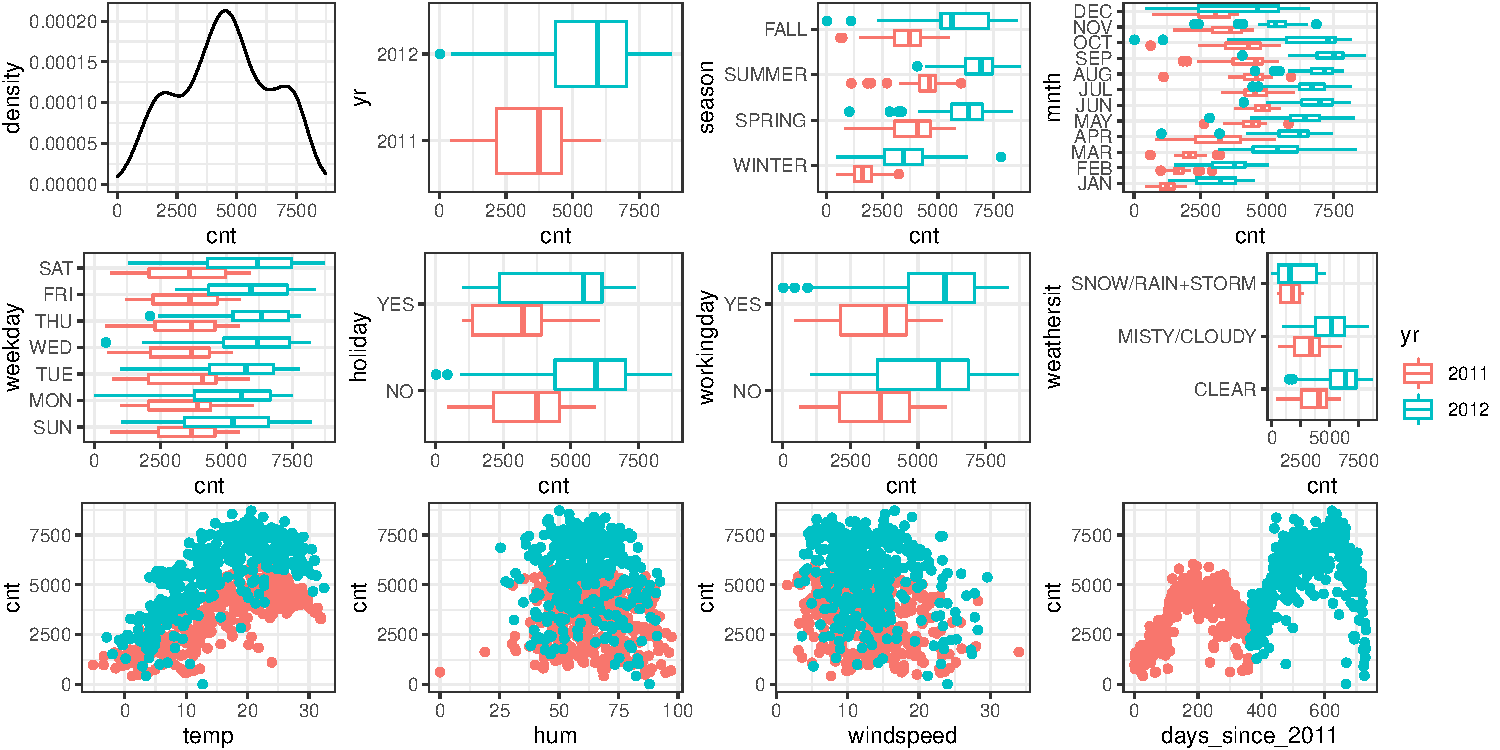
\includegraphics[width=\linewidth]{figure/intro_bike}
\end{frame}

\endlecture
\end{document}
